\documentclass[a4paper, 12pt, final, garamond]{book}
\usepackage{cours-preambule}

\raggedbottom

\makeatletter
\renewcommand{\@chapapp}{M\'ecanique -- chapitre}
\makeatother

\begin{document}
\setcounter{chapter}{4}

\chapter{TD application~: mouvement de particules charg\'ees}

\section{Mouvements simples de particules chargées}

On considère une particule ponctuelle, de charge $q$ et de masse $m$, de vitesse
initiale $\vfo$ à l'entrée d'une zone où règnent un champ électrique $\Ef$ ou un
champ magnétique $\Bf$. On suppose ces champs uniformes et indépendants du
temps, et on néglige toute autre force que celles provoquées par ces champs.

On suppose dans un premier temps que la particule décrit une droite et possède
une accélération constante $a$. \bigbreak

\begin{enumerate}
    \item Déterminer la direction et la norme du ou des champs qui provoquent
        cette trajectoire.
    \item Déterminer la position $\OM$ du point en fonction du temps. On
        notera $\OM_0$ la position initiale.
\end{enumerate} \bigbreak

La particule décrit maintenant une trajectoire circulaire de rayon $R_0$, dans
un plan $x\Or y$. \bigbreak

\begin{enumerate}[resume]
    \item Déterminer la direction du ou des champs qui provoquent cette
        trajectoire.
    \item Déterminer l'équation de la trajectoire et la relation entre la norme
        du champ, $v_0$ et $R_0$. On suggère d'utiliser les coordonnées
        polaires.
\end{enumerate}

\section{Filtre de vitesse}

\begin{minipage}[c]{0.50\linewidth}
    Un ion de masse $m$ et de charge $q$ pénètre dans un filtre par la fente $F_1$
    avec un vecteur vitesse $\vf = v_0\ux$. Il y règne un champ électrique $\Ef =
    E\uy$ et un champ magnétique $\Bf$ = $B\uz$, uniformes et stationnaires.
\end{minipage}
\hfill
\begin{minipage}[c]{0.50\linewidth}
    \begin{center}
        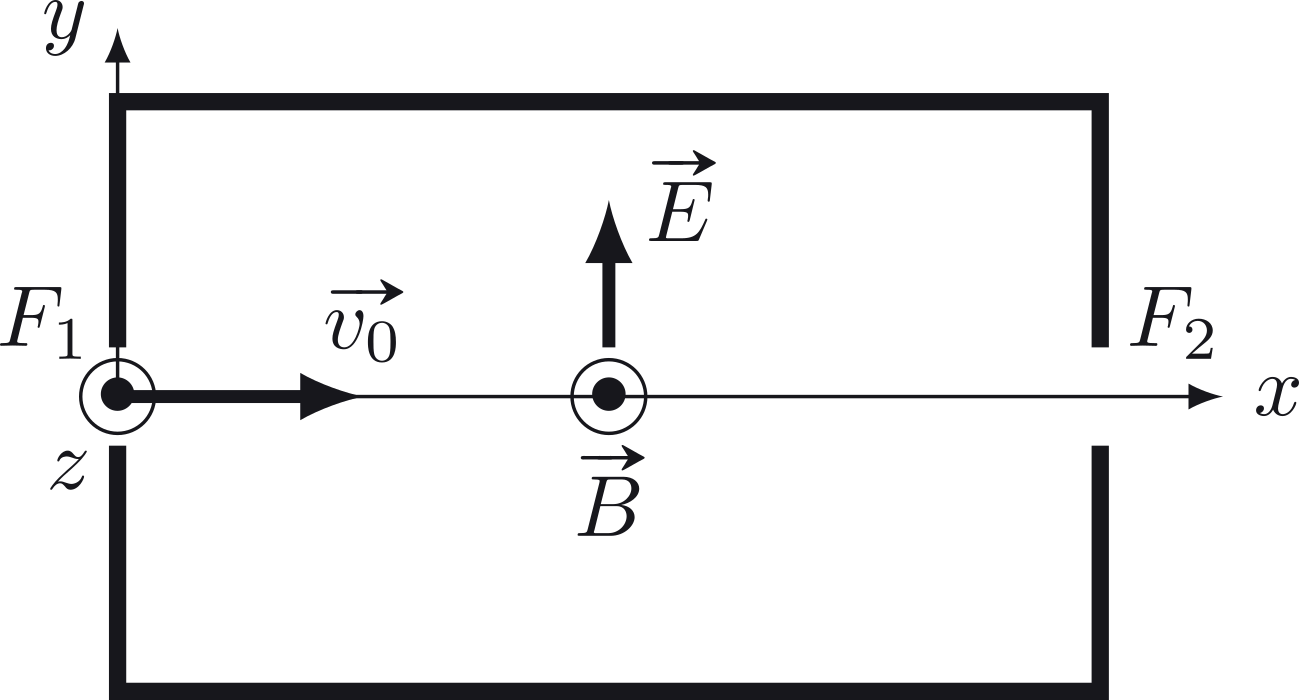
\includegraphics[width=5cm]{filtre_vitesse-plain}
        \captionof{figure}{Schéma du filtre de vitesse.}
        \label{fig:fdv}
    \end{center}
\end{minipage}
\hfill~

\begin{enumerate}
    \item Écrire la force de \textsc{Lorentz} alors ressentie par l'ion.
    \item À quelle condition l'ion peut-il avoir une trajectoire rectiligne
        l'amenant à passer à travers la fente $F_2$~?
    \item Exprimer en fonction de $E$ et $B$ la vitesse $v_0$ lui permettant
        d'atteindre la fente $F_2$. Justifier le nom du dispositif.
\end{enumerate}

\section{Déviation d'un électron}

\begin{minipage}[c]{0.50\linewidth}
    Un électron pénètre en $A$ avec une vitesse initiale $\vfo$ dans la zone
    grisée où règne un champ magnétique $\Bf$ uniforme et stationnaire. On
    suppose que la zone où règne le champ magnétique est très grand de telle
    sorte que la particule ne peut que ressortir par les côtés AC ou AD. 
\end{minipage}
\hfill
\begin{minipage}[c]{0.50\linewidth}
    ~
    \begin{center}
        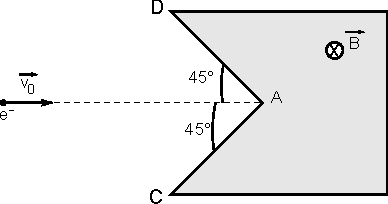
\includegraphics[width=5cm]{miroir_mag-plain}
        \captionof{figure}{Schéma de la situation.}
        \label{fig:mirmag}
    \end{center}
\end{minipage}

\begin{enumerate}
    \item Quelle est la trajectoire de la particule dans la zone grisée~? On
        précisera les caractéristiques de cette trajectoire.
    \item Par quelle face ressort la particule~? Quelle est la direction de la
        vitesse~?
    \item Que se passe-t-il ensuite~? Quel nom donneriez-vous à ce dispositif~?
\end{enumerate}

\section{Imprimante jet d'encre}

Dans un dispositif d'impression industriel, les gouttelettes d'encre sont
chargées puis déviées de manière contrôlée par un déflecteur électrostatique
avant d'atteindre le support d'impression. \bigbreak

\begin{minipage}[t]{0.45\linewidth}
    Un gouttelette de volume $V = \SI{10}{pL}$, de charge $q = \SI{3.4e-14}{C}$
    et de vitesse $v_0 = \SI{20}{m.s^{-1}}$ entre en O dans le déflecteur,
    constitué de deux électrodes planes portées aux potentiels électriques $V_1$
    et $V_2$ et générant un champ électrostatique uniforme $\Ef = E\uy$ avec $E
    = \SI{5.0e5}{V.m^{-1}}$. \bigbreak
    La longueur du déflecteur est $L_1 = \SI{5.0}{cm}$. Le support d'impression
    se trouve à la distance $L_2 = \SI{20}{cm}$ de la sortie du déflecteur.
    L'encre est essentiellement constituée d'eau, de masse volumique $\rho =
    \SI{1.0e3}{kg.m^{-3}}$.
\end{minipage}
\hfill
\begin{minipage}[t]{0.45\linewidth}
    ~\vspace{-12pt}
    \begin{center}
        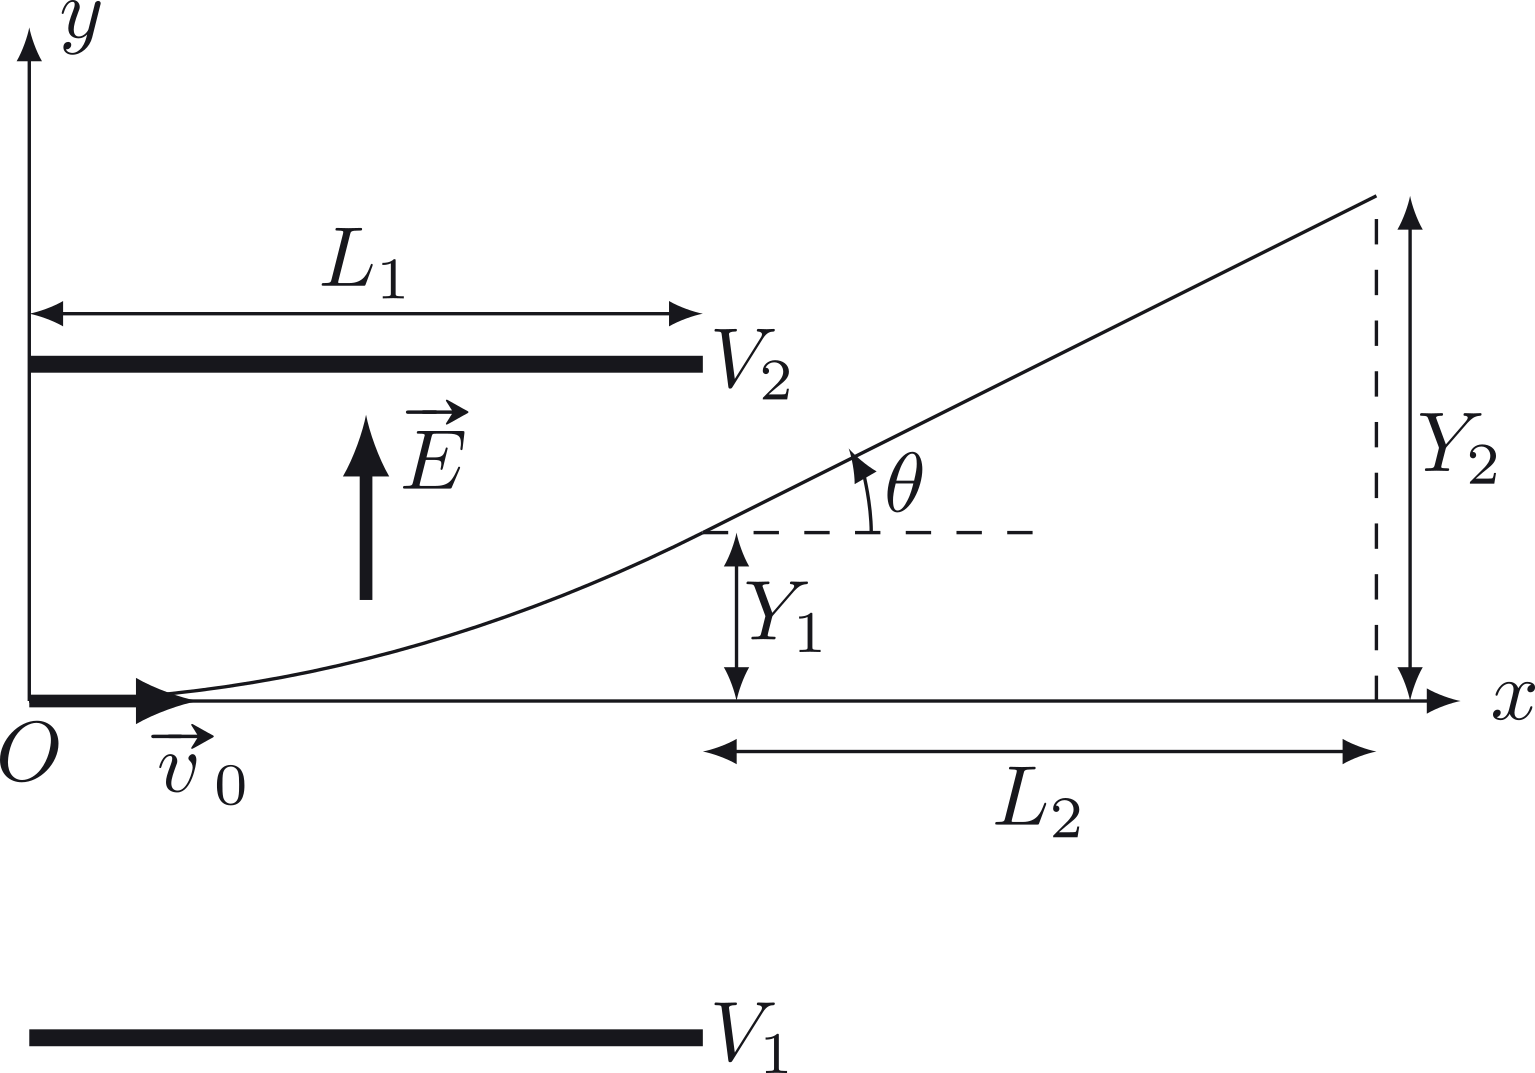
\includegraphics[width=\linewidth]{deflecteur_plain}
        \captionof{figure}{Schéma du déflecteur.}
        \label{fig:deflec}
    \end{center}
\end{minipage}\bigbreak

\begin{enumerate}
    \item Quel est le signe de la tension $V_1 - V_2$ pour que la gouttelette
        d'encre soit effectivement déviée dans le sens des $y$ croissants~?
    \item Calculer la masse $m$ de la gouttelette et montrer que l'on peut
        négliger son poids devant la force électrique de \textsc{Lorentz}.
    \item Appliquer la deuxième loi de \textsc{Newton} à la gouttelette entre
        les électrodes et déterminer l'équation de sa trajectoire. En déduire le
        déplacement $Y_1$ en sortie du déflecteur.
    \item Caractériser la trajectoire de la gouttelette après sa sortie du
        déflecteur, en négligeant son poids.
    \item Exprimer puis calculer la déflexion angulaire $\tt$. En déduire le
        déplacement $Y_2$.
\end{enumerate}

\end{document}
